\documentclass{article}
\usepackage[a4paper, margin=1in,paperheight=15in,paperwidth=9in]{geometry}
\usepackage[utf8]{inputenc}
\usepackage{amsmath}
\usepackage{graphicx}

\title{Numerical Analysis Homework 1}
\author{131044009 - Hasan MEN}
\date{12 March 2017}

\begin{document}

\maketitle

\section{Q1: Section 2.1 exercise 6}

\begin{figure}[h]
       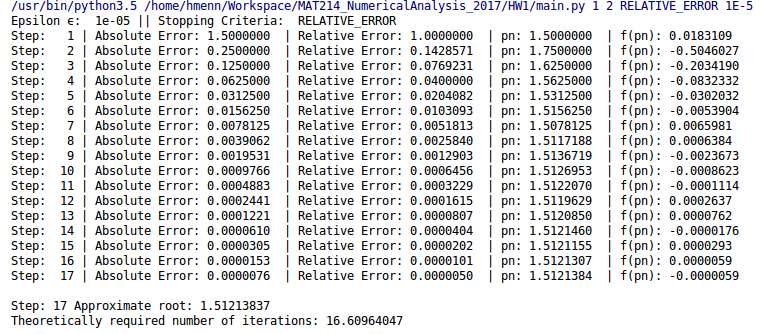
\includegraphics[width=400px]{ss_2_2_6_a.png}
       \caption{a}
\end{figure}
There is no valid root between 0 and 1. If we draw pilot, we will see root between 1-2.
\begin{figure}[h]
       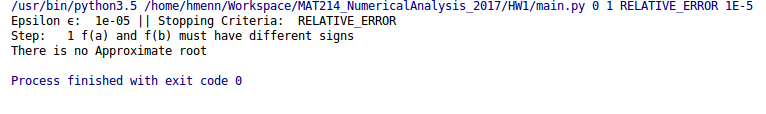
\includegraphics[width=400px]{ss_2_2_6_b.png}
       \caption{b}
\end{figure}
\begin{figure}[h]
       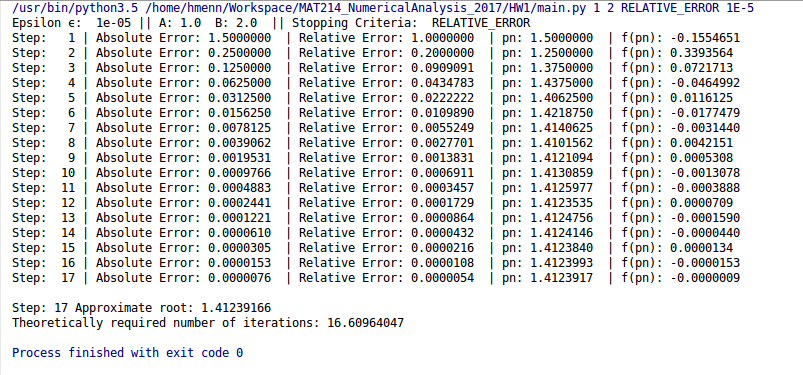
\includegraphics[width=400px,height=200px]{ss_2_2_6_c_1.png}
       \caption{c1}
\end{figure}
\begin{figure}[h]
       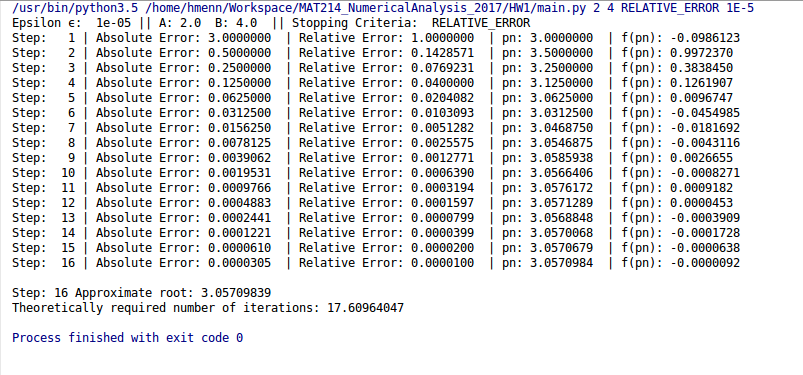
\includegraphics[width=400px,height=200px]{ss_2_2_6_c_2.png}
       \caption{c2}
\end{figure}
\newpage
\begin{figure}[h]
       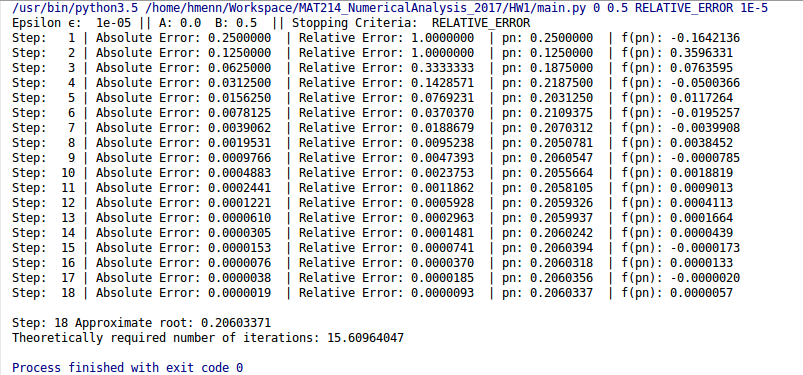
\includegraphics[width=400px]{ss_2_2_6_d_1.png}
       \caption{d1}
\end{figure}
\begin{figure}[h]
       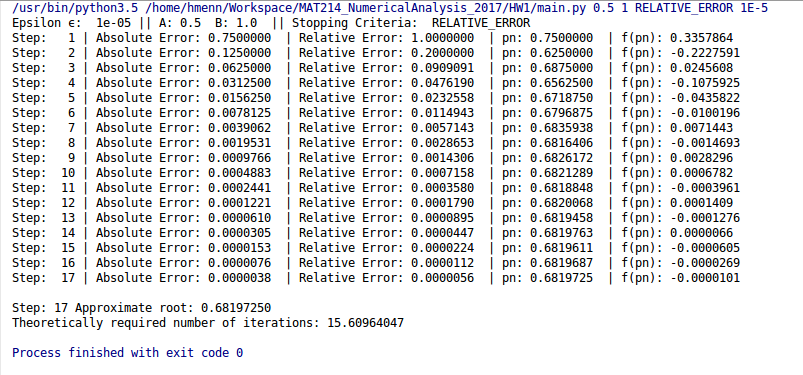
\includegraphics[width=400px]{ss_2_2_6_d_2.png}
       \caption{d2}
\end{figure}
\newpage
\section{Q2: Section 2.2 exercise 5}
If g is defined on [a, b] and g(p) = p for some p $\in$ [a, b], then the function g is said to have the fixed point p in [a, b].\\

Use a fixed-point iteration method to determine a solution accurate to within $10^{-2}$ for $x^4-3*x^2-3 = 0$ on $[1, 2]$. Use $p_0 = 1$.
\subsection{Answer}
Firstly, manipulate function to obtain $x=g(x)$
\begin{align}
\label{2.2.5.1}
g(x) & = x^4-3*x^2-3 = 0\\
\label{2.2.5.2}
x^4 & = 3*x^2+3\\
\label{2.2.5.3}
x & = (3*x^2+3)^ \frac{1}{4}=g(x)
\end{align}
Let's substitute $p_0=1$ in function to calculate $p_1=?$\\
\begin{align}
\label{2.2.5.4}	p_1 & = g(p_0)\\
\label{2.2.5.5}	p_1 & = (3*1^2+3)^ \frac{1}{4}\\
\label{2.2.5.6} p_1 & = 1.5650846
\end{align}
Next step, find absolute difference between two points($p_0$ and $p_1$)\ to make a comparison with $\varepsilon = 10^{-2}$\\\\
if $|p_1-p_0|< \epsilon$ return $p_1$\\
else set $p_0=p_1$ and go step \ref{2.2.5.4}
\begin{align}
\label{2.2.5.7} |p_1-p_0| & = 1.5650846 - 1.0 = 0.5650846 \\
\label{2.2.5.8} |p_1-p_0| & > \epsilon=10^{-2}
\end{align}

Set $p_0$ to $p_1$ and go step. Calculate all steps until find a good approximate value.\\

\begin{tabular}{r|cc|l}
step(i) & $p_(i-1)$ & $p_i$ & $|p_0-p_i|$\\
\hline
1 & 1.0000000 & 1.5650846 & 0.5650846\\
2 & 1.5650846 & 1.7935729 & 0.2284883\\
3 & 1.7935729 & 1.8859437 & 0.0923709\\
4 & 1.8859437 & 1.9228478 & 0.0369041\\
5 & 1.9228478 & 1.9375075 & 0.0146597\\
6 & 1.9375075 & 1.9433169 & 0.0058094\\
\end{tabular}
Result: $p_6= 1.9433169$\\

\textbf{Theoretically number of iteration:}
\begin{align}
\label{k}|p-p_n| & \leq\frac{k^n}{1-k}*|p_1-p_0|\\
\label{}g'(x) \approx k & = ((3*x^2+3)^ \frac{1}{4})'\\
\label{}g'(x) \approx k & = (1.5*x*(3*x^2+3))^ \frac{-3}{4}\\
\label{}g'(1) \approx k & = 0.391\\
\label{}|p-p_n| & \leq\frac{(0.391)^n}{1-0.391}*|1.5650846-1|\\
\label{}& \leq\frac{(0.391)^n}{0.609}*|0.5650846|\\
\label{} (0.391)^n*0,92788 & < 10^{-2} \\
\label{} n& \approx 6
\end{align}
\section{Q3: Section 2.3 exercise 4}
Let $f(x)=-x^3-cos(x)$. With $p_0 =-1$ and $p_1 = 0$, find $p_3$.\\
a. Use the Secant method. b. Use the method of False Position.
\subsection{a. Secant Method}
$f(0)=-1, f(-1)=0.4596976$
\begin{align}
\label{secant_theorem}p_n & = p_{n-1}-\frac{f(p_{n-1})(p_{n-1}-p_{n-2})}{f(p_{n-1})-f(p_{n-2})}\\
\label{2.3.a.1}p_3 & = p_2 - \frac{f(p_2)(p_2-p_1)}{f(p_2)-f(p_1)}\\
\label{2.3.a.2}p_2 & = p_1 - \frac{f(p_1)(p_1-p_0)}{f(p_1)-f(p_0)}\\
\label{2.3.a.3}p_2 & = 0 - \frac{f(0)(0-(-1))}{f(0)-f(-1)}\\
\label{2.3.a.4}p_2 & = \frac{1}{-1-(0.4596976)}\\
\label{2.3.a.5}p_2 & = -0.6850733\\
\end{align}
Substitute $p_2$ to step(\ref{2.3.a.1})
\begin{align}
\label{2.3.a.6}p_3 & = (-0.6850733) - \frac{f(-0.6850733)(-0.6850733-0)}{f(-0.6850733)-f(0)}\\
\label{2.3.a.7}p_3 & = -1.2520764
\end{align}

\subsection{b. The Method of False Position}
$p_0=-1, p_1=0, f(0)=-1, f(-1)=0.4596976$
\begin{align}
\label{2.3.b.1}p_n & = p_{n-1} - q_{n-1}\frac{p_{n-1}-p_{n-2}}{f(p_{n-1})-f(p_{n-2}))}\\
\label{2.3.b.2}p_3 & = p_2 - q_2\frac{p_2-p_1}{f(p_2)-f(p_1))}\\
\label{2.3.b.3}p_2 & = p_1 - q_1\frac{p_1-p_0}{f(p_1)-f(p_0))}\\
\label{2.3.b.3.1}q_1 & = f(p_1)\\
\label{2.3.b.4}p_2 & = 0 - f(p_1)\frac{0-(-1)}{f(0)-f(-1)}\\
\label{2.3.b.5}p_2 & = -0.68507335\\
\end{align}
Substitute $p_2$ to step(\ref{2.3.b.2})

\begin{align}
\label{2.3.b.6}p_3 & = p_2 - f(p_2)\frac{p_2-p_1}{f(p_2)-f(p_1))}\\
\label{2.3.b.7}p_3 & = -0.841355125
\end{align}


\section{Q3: Section 2.3 exercise 5}
Use Newton’s method to find solutions accurate to within $10^{-4}$ for the following problems.\\
Newton's Method
\begin{align}
\label{newton_method} p_n & = p_{n-1} - \frac{f(p_{n-1})}{f'(p_{n-1})}
\end{align}
\subsection{a. $f(x)=x^3-2*x^2-5 = 0, [1, 4]$}
\begin{equation}
f'(x)=3*x^2-4*x
\end{equation}
Let's take $p_0=2$ and $\epsilon=10^{-2}$
\begin{align}
\label{2.3.5.a.1}p_1 & = p_0 - \frac{f(p_0)}{f'(p_o)}\\
\label{2.3.5.a.2}p_1 & = 2 - \frac{f(2)}{f'(2)}\\
\label{2.3.5.a.3}p_1 & = 3.2500000\\
\label{2.3.5.a.4}|p_1-p_0| & =1.250000 > \epsilon
\end{align}
$p_1$ has not enough approximate value. Calculate $p_2$
\begin{align}
\label{2.3.5.a.5}p_2 & = p_1 - \frac{f(p_1)}{f'(p_1)}\\
\label{2.3.5.a.6}p_2 & = 3.25 - \frac{f(3.25)}{f'(3.25)}\\
\label{2.3.5.a.7}p_2 & = 2.8110368\\
\label{2.3.5.a.8}|p_2-p_1| & =0.4389632 > \epsilon
\end{align}
$p_2$ has not enough approximate value. Calculate $p_3$
\begin{align}
\label{2.3.5.a.9}p_3 & = p_2 - \frac{f(p_2)}{f'(p_2)}\\
\label{2.3.5.a.10}p_3 & = 2.8110368 - \frac{f(2.8110368)}{f'(2.8110368)}\\
\label{2.3.5.a.11}p_3 & = 2.6979895\\
\label{2.3.5.a.12}|p_3-p_2| & =0.1130473 > \epsilon
\end{align}
$p_3$ has not enough approximate value. Calculate $p_4$
\begin{align}
\label{2.3.5.a.13}p_4 & = p_3 - \frac{f(p_3)}{f'(p_3)}\\
\label{2.3.5.a.14}p_4 & = 2.6979895 - \frac{f(2.6979895)}{f'(2.6979895)}\\
\label{2.3.5.a.15}p_4 & = 2.6906772\\
\label{2.3.5.a.16}|p_4-p_3| & =0.0073123 > \epsilon
\end{align}
$p_4$ has not enough approximate value. Calculate $p_5$
\begin{align}
\label{2.3.5.a.17}p_5 & = p_4 - \frac{f(p_4)}{f'(p_4)}\\
\label{2.3.5.a.18}p_5 & = 2.6906772 - \frac{f(2.6906772)}{f'(2.6906772)}\\
\label{2.3.5.a.19}p_5 & = 2.6906474\\
\label{2.3.5.a.20}|p_5-p_4| & =0.0000297 < \epsilon
\end{align}
Answer is $p_5:2.6906474$ and $1\leq p_5 \leq 4$. Founded in 5.step

\subsection{b. $f(x)=x^3+2*x^2-1 = 0, [-3, -2]$}
\begin{equation}
f'(x)=3*x^2+4*x
\end{equation}
Let's take $p_0=-3$ and $\epsilon=10^{-2}$
\begin{align}
\label{2.3.5.b.1}p_1 & = p_0 - \frac{f(p_0)}{f'(p_o)}\\
\label{2.3.5.b.2}p_1 & = -3 - \frac{f(-3)}{f'(-3)}\\
\label{2.3.5.b.3}p_1 & = -2.8888889\\
\label{2.3.5.b.4}|p_1-p_0| & =0.1111111 > \epsilon
\end{align}
$p_1$ has not enough approximate value. Calculate $p_2$
\begin{align}
\label{2.3.5.b.1}p_2 & = p_1 - \frac{f(p_1)}{f'(p_1)}\\
\label{2.3.5.b.2}p_2 & = -2.8888889 - \frac{f(-2.8888889)}{f'(-2.8888889)}\\
\label{2.3.5.b.3}p_2 & = -2.8794516\\
\label{2.3.5.b.4}|p_2-p_1| & =0.0094373 > \epsilon
\end{align}
$p_2$ has not enough approximate value. Calculate $p_3$
\begin{align}
\label{2.3.5.b.1}p_3 & = p_2 - \frac{f(p_2)}{f'(p_2)}\\
\label{2.3.5.b.2}p_3 & = -2.8794516 - \frac{f(-2.8794516)}{f'(-2.8794516)}\\
\label{2.3.5.b.3}p_3 & = -2.8793852\\
\label{2.3.5.b.4}|p_3-p_2| & =0.0000663 < \epsilon
\end{align}

Answer is $p_3:-2.8793852$ and $-3\leq p_3 \leq -2$. Founded in 3.step

\subsection{c. $f(x)=x-cos(x) = 0, [0, \frac{\pi}{2}]$}
\begin{equation}
f'(x)=1+sin(x)
\end{equation}
Let's take $p_0=0$ and $\epsilon=10^{-2}$
\begin{align}
\label{2.3.5.c.1}p_1 & = p_0 - \frac{f(p_0)}{f'(p_o)}\\
\label{2.3.5.c.2}p_1 & = 0 - \frac{f(0)}{f'(0)}\\
\label{2.3.5.c.3}p_1 & = 1.0000000\\
\label{2.3.5.c.4}|p_1-p_0| & =1.0000000 > \epsilon
\end{align}
$p_1$ has not enough approximate value. Calculate $p_2$
\begin{align}
\label{2.3.5.c.1}p_2 & = p_1 - \frac{f(p_1)}{f'(p_1)}\\
\label{2.3.5.c.2}p_2 & = 1.0000000 - \frac{f(1.0000000)}{f'(1.0000000)}\\
\label{2.3.5.c.3}p_2 & = 0.7503639\\
\label{2.3.5.c.4}|p_2-p_1| & =0.2496361 > \epsilon
\end{align}
$p_2$ has not enough approximate value. Calculate $p_3$
\begin{align}
\label{2.3.5.c.1}p_3 & = p_2 - \frac{f(p_2)}{f'(p_2)}\\
\label{2.3.5.c.2}p_3 & = 0.7503639 - \frac{f(0.7503639)}{f'(0.7503639)}\\
\label{2.3.5.c.3}p_3 & = 0.7391129\\
\label{2.3.5.c.4}|p_3-p_2| & =0.0112510 > \epsilon
\end{align}
$p_3$ has not enough approximate value. Calculate $p_4$
\begin{align}
\label{2.3.5.c.1}p_4 & = p_3 - \frac{f(p_3)}{f'(p_3)}\\
\label{2.3.5.c.2}p_4 & = 0.739112 - \frac{f(0.739112)}{f'(0.739112)}\\
\label{2.3.5.c.3}p_4 & = 0.7390851\\
\label{2.3.5.c.4}|p_4-p_3| & =0.0000278 < \epsilon
\end{align}

Answer is $p_4:0.7390851$ and $0\leq p_4 \leq \frac{\pi}{2}$. Founded in 4.step\\\\

\subsection{d. $f(x)=x-0.8-0.2*sin(x) = 0, [0,\frac{\pi}{2}]$}
\begin{equation}
f'(x)=1-0.2*cos(x)
\end{equation}
Let's take $p_0=0$ and $\epsilon=10^{-2}$
\begin{align}
\label{2.3.5.d.1}p_1 & = p_0 - \frac{f(p_0)}{f'(p_o)}\\
\label{2.3.5.d.2}p_1 & = 0 - \frac{f(0)}{f'(0)}\\
\label{2.3.5.d.3}p_1 & = 1.0000000\\
\label{2.3.5.d.4}|p_1-p_0| & =1.0000000 > \epsilon
\end{align}
$p_1$ has not enough approximate value. Calculate $p_2$
\begin{align}
\label{2.3.5.d.1}p_2 & = p_1 - \frac{f(p_1)}{f'(p_1)}\\
\label{2.3.5.d.2}p_2 & = 1.0000000 - \frac{f(1.0000000)}{f'(1.0000000)}\\
\label{2.3.5.d.3}p_2 & = 0.9644530\\
\label{2.3.5.d.4}|p_2-p_1| & =0.0355470 > \epsilon
\end{align}
$p_2$ has not enough approximate value. Calculate $p_3$
\begin{align}
\label{2.3.5.d.1}p_3 & = p_2 - \frac{f(p_2)}{f'(p_2)}\\
\label{2.3.5.d.2}p_3 & = 0.9644530 - \frac{f(0.9644530)}{f'(0.9644530)}\\
\label{2.3.5.d.3}p_3 & = 0.9643339\\
\label{2.3.5.d.4}|p_3-p_2| & =0.0001191 < \epsilon
\end{align}

Answer is $p_3:0.9643339$ and $0\leq p_3 \leq \frac{\pi}{2}$. Founded in 3.step


\end{document}

